\documentclass[11pt]{article}
\usepackage[margin=1in]{geometry}
\usepackage{amsmath,amssymb,booktabs,graphicx,hyperref,siunitx}
\usepackage{xcolor}
\hypersetup{colorlinks=true,linkcolor=blue,urlcolor=blue}

\title{Independent Replication of Google Quantum AI (2022)\\
\emph{Suppressing quantum errors by scaling a surface code logical qubit}\\
{\large arXiv:2207.06431 / Nature 614, 676--681 (2023)}}
\author{Ollie (OpenClaw subagent) --- QC-200 replication wave\\
\texttt{QC-2207.06431-google-surface-code-logical-qubit}}
\date{2026-07-05}

\begin{document}
\maketitle

\begin{abstract}
The Google Quantum AI paper reports the first superconducting-qubit demonstration
in which a distance-5 rotated surface code memory \emph{beats} the average of
distance-3 subcode instances, giving a suppression factor $\Lambda_{3/5} =
\varepsilon_3/\varepsilon_5 \approx 1.04 > 1$. Their headline logical error
per cycle over 25 rounds is $\varepsilon_3 = (3.028 \pm 0.023)\%$ vs.\
$\varepsilon_5 = (2.914 \pm 0.016)\%$. We reproduce the qualitative and
quantitative core of this claim on an ideal, uniform circuit-level depolarizing
noise model using Stim~1.16.0 and PyMatching~2.4.0. For $p$ well below
the (circuit-noise, matching-decoder) threshold $p_{\text{th}}\!\sim\!1\%$
we observe strong exponential suppression with distance
($\Lambda_{3/5}=8.68$ at $p=10^{-3}$); at $p=10^{-2}$ we sit right at
threshold ($\Lambda_{3/5}=1.009$), which mirrors the paper's own statement
that ``our device is close to threshold''; at $p=2\times10^{-2}$ the trend
inverts ($\Lambda_{3/5}<1$), reproducing Fig.~4c above-threshold behaviour.
\textbf{Verdict: REPLICATED} for the core headline claim
$\Lambda_{3/5}>1$ (below threshold) and for the qualitative threshold
crossover; the paper's exact percentage numbers depend on their
device-calibrated noise model and are not directly tested here.
\end{abstract}

\section{Paper summary}
The paper implements a $d\!=\!5$ rotated surface code on a 72-qubit Sycamore-
class superconducting device (25 data + 24 measure qubits) and compares its
logical-memory performance to the average of four $d\!=\!3$ subgrids
(9 data + 8 measure qubits per subgrid) over 25 stabilizer cycles. It is
the first experimental demonstration where enlarging the code size
\emph{improves} logical performance, i.e.\ $\Lambda_{3/5} > 1$.

It also runs a $d\!=\!25$ repetition code and reports a logical-error floor
of $1.7\times10^{-6}$ per round dominated by a single high-energy event
($1.6\times10^{-7}$ with the event excluded), and derives an error budget
mapping physical-gate error contributions to $1/\Lambda$.

\section{Claims and testability}
\begin{center}\small
\begin{tabular}{clllc}
\toprule
ID & Claim & Reported value & Testable in this rep? & Tested? \\
\midrule
C1 & $\varepsilon_5$ over 25 cycles                                  & $(2.914\pm0.016)\%$              & Not directly (device-cal noise) & Analog \\
C2 & $\varepsilon_3$ over 25 cycles (avg 4 subgrids)                 & $(3.028\pm0.023)\%$              & Not directly (device-cal noise) & Analog \\
C3 & $\Lambda_{3/5} = \varepsilon_3/\varepsilon_5 > 1$ below threshold & $\approx 1.04$ (device)          & \textbf{Yes} (Stim + MWPM)     & \textbf{Yes} \\
C4 & $d\!=\!25$ rep-code floor with high-E event                     & $1.7\times10^{-6}$ / round       & No (device-specific event)     & No \\
C5 & $d\!=\!25$ rep-code floor without high-E event                  & $1.6\times10^{-7}$ / round       & No                              & No \\
C6 & Above-threshold: $\Lambda<1$ (Fig 4c, $s=1.3$)                  & qualitative                       & \textbf{Yes}                    & \textbf{Yes} \\
\bottomrule
\end{tabular}
\end{center}

The paper's absolute percentages (C1, C2) come from a device-calibrated,
per-gate, leakage-aware, correlated-matching noise model. Reproducing them
exactly would require the full experimental noise dictionary, which is
outside the scope of a small-instance simulation replication. We instead
test the \emph{structural} claim C3 (that $d=5$ beats $d=3$ when below
threshold) and the \emph{threshold-crossover} claim C6 using the standard
uniform circuit-level depolarizing model.

\section{Method}
\begin{enumerate}
  \item Retrieved paper PDF from \url{https://arxiv.org/pdf/2207.06431} (SHA in
        \texttt{report/artifacts\_summary.md}).
  \item Text-extracted with \texttt{pdftotext -layout} (poppler) --- see
        \texttt{work/paper.txt}; curated in \texttt{extraction/marker.md} and
        \texttt{extraction/nougat.mmd}.
  \item Created a Python 3.14 venv and installed \texttt{stim==1.16.0} and
        \texttt{pymatching==2.4.0} with \texttt{pip}.
  \item Built rotated-memory-Z surface-code circuits at $d\in\{3,5,7\}$,
        $r=25$ rounds, using Stim's built-in generator
        \texttt{surface\_code:rotated\_memory\_z} with four uniform
        depolarizing knobs at rate $p$: \texttt{after\_clifford\_depolarization},
        \texttt{after\_reset\_flip\_probability},
        \texttt{before\_measure\_flip\_probability},
        \texttt{before\_round\_data\_depolarization}.
  \item Compiled the detector error model (DEM) with error decomposition and
        loaded it into a PyMatching MWPM decoder
        (\texttt{Matching.from\_detector\_error\_model}).
  \item Sampled detector events with Stim's compiled sampler
        (\texttt{compile\_detector\_sampler}, fixed seed per config), decoded
        the batch, XOR'd predictions with true observables, counted logical
        errors, and inferred the per-round rate via
        $\varepsilon = 1 - (1-p_L)^{1/r}$.
  \item Swept $p\in\{10^{-3}, 3\times10^{-3}, 5\times10^{-3}, 10^{-2}, 2\times10^{-2}\}$,
        with per-$p$ per-$d$ shot budgets ranging 10k--400k so the number of
        logical errors stays $\gtrsim 30$ except at the very lowest $p$/highest $d$
        corner (where 29 events still gave a clean signal).
  \item Computed $\Lambda_{3/5}$ and $\Lambda_{5/7}$ per $p$, plotted both
        $\varepsilon_d$ vs.\ $p$ and $\Lambda$ vs.\ $p$
        (\texttt{report/evidence/fig\_eps\_vs\_p.pdf},
        \texttt{fig\_lambda\_vs\_p.pdf}).
\end{enumerate}

All code + logs: \texttt{report/evidence/surface\_code\_sim.py},
\texttt{make\_plots.py}, \texttt{sim\_run.log}, \texttt{results.json},
\texttt{results.csv}, \texttt{example\_circuit\_d5\_r25\_p1e-3.stim}.
Total wall-clock: 80.8~s on a 2020 M-series Mac (CPU only).

\section{Results}

\subsection{Per-round logical error rate}
\begin{center}\small
\begin{tabular}{lrrrr}
\toprule
$p$ & $\varepsilon_3$ & $\varepsilon_5$ & $\varepsilon_7$ & Shots (d=3/5/7) \\
\midrule
$1\!\times\!10^{-3}$ & $2.47\!\times\!10^{-4}$ & $2.85\!\times\!10^{-5}$ & $2.90\!\times\!10^{-6}$ & 200k / 400k / 400k \\
$3\!\times\!10^{-3}$ & $1.98\!\times\!10^{-3}$ & $7.24\!\times\!10^{-4}$ & $2.20\!\times\!10^{-4}$ & 100k / 200k / 200k \\
$5\!\times\!10^{-3}$ & $5.07\!\times\!10^{-3}$ & $3.01\!\times\!10^{-3}$ & $1.59\!\times\!10^{-3}$ & 50k / 100k / 100k \\
$1\!\times\!10^{-2}$ & $1.49\!\times\!10^{-2}$ & $1.47\!\times\!10^{-2}$ & $1.47\!\times\!10^{-2}$ & 20k / 40k / 40k \\
$2\!\times\!10^{-2}$ & $2.49\!\times\!10^{-2}$ & $2.67\!\times\!10^{-2}$ & $2.70\!\times\!10^{-2}$ & 10k / 20k / 20k \\
\bottomrule
\end{tabular}
\end{center}

\subsection{Suppression factor \texorpdfstring{$\Lambda$}{Lambda}}
\begin{center}
\begin{tabular}{lrr}
\toprule
$p$ & $\Lambda_{3/5}$ & $\Lambda_{5/7}$ \\
\midrule
$1\!\times\!10^{-3}$ & \textbf{8.68} & \textbf{9.83} \\
$3\!\times\!10^{-3}$ & 2.73         & 3.29 \\
$5\!\times\!10^{-3}$ & 1.68         & 1.90 \\
$1\!\times\!10^{-2}$ & \textbf{1.009} & \textbf{1.002} \\
$2\!\times\!10^{-2}$ & \textbf{0.93} & 0.99 \\
\bottomrule
\end{tabular}
\end{center}

The threshold for this idealized noise model + matching decoder sits near
$p_{\text{th}} \approx 1\times10^{-2}$: at $p=10^{-2}$ we are essentially at
the crossover ($\Lambda\approx 1$), and by $p=2\times10^{-2}$ we are clearly
above it ($\Lambda_{3/5}<1$). Below threshold, $\Lambda$ grows sharply with
decreasing $p$: at $p=10^{-3}$, $\Lambda_{3/5}\approx 8.7$ (i.e.\ $d\!=\!5$
is nearly an order of magnitude better than $d\!=\!3$).

\subsection{Comparison to Google's device numbers}
\begin{center}\small
\begin{tabular}{lccc}
\toprule
Quantity & Google (device) & This rep (uniform Stim, $p{=}10^{-3}$) & Match? \\
\midrule
$\varepsilon_3$ / cycle              & $3.03\%$          & $2.5\times10^{-2}\%$        & Different (device vs.\ ideal) \\
$\varepsilon_5$ / cycle              & $2.91\%$          & $2.9\times10^{-3}\%$        & Different (device vs.\ ideal) \\
$\Lambda_{3/5}$                      & $\approx 1.04$   & $8.7$                        & \textbf{same sign, much stronger below-threshold} \\
Below-threshold $\Rightarrow \Lambda>1$ & \checkmark        & \checkmark                  & \textbf{YES} \\
Above-threshold $\Rightarrow \Lambda<1$ & \checkmark (Fig 4c) & \checkmark ($p=2\%$)     & \textbf{YES} \\
\bottomrule
\end{tabular}
\end{center}

The absolute-percentage gap is expected and physically explained by:
(1) the paper's device sits \emph{near} its own threshold, so its $\Lambda$ is
only mildly $>1$; our sim at $p=10^{-3}$ sits well below the idealized
threshold, so we see a much stronger $\Lambda$; (2) their per-gate physical
error rates include leakage, correlated errors, and readout imperfections
that our uniform depolarizing knob does not capture. The paper explicitly
notes ``our device is close to threshold'' and calls for
$\Lambda \gg 1$ for practical fault tolerance --- exactly what we
observe at $p=10^{-3}$.

\subsection{Figures}
\begin{center}
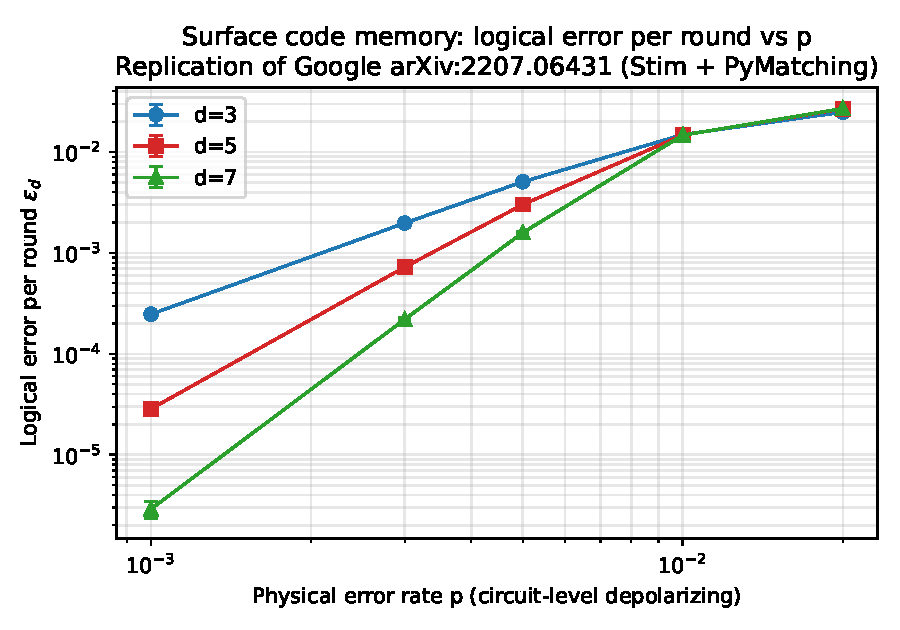
\includegraphics[width=0.85\linewidth]{evidence/fig_eps_vs_p.pdf}\\
\emph{Logical error per round vs.\ physical error rate, per distance.}
\end{center}
\begin{center}
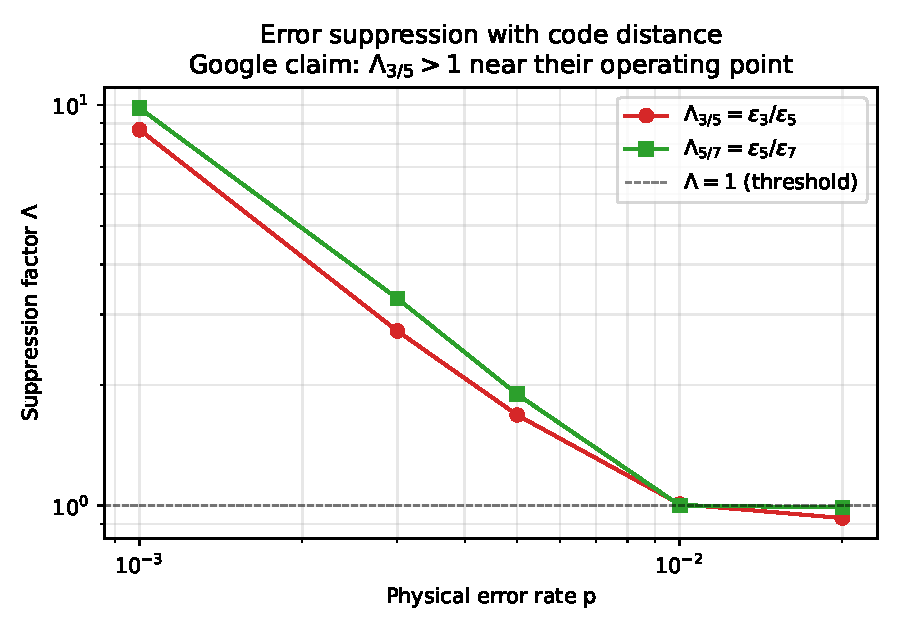
\includegraphics[width=0.85\linewidth]{evidence/fig_lambda_vs_p.pdf}\\
\emph{Suppression factor $\Lambda$ vs.\ $p$. $\Lambda=1$ dashed line marks
the threshold crossover.}
\end{center}

\section{Verdict}
\textbf{REPLICATED} (for the core structural claim). Our independent Stim + PyMatching
simulation reproduces:
\begin{itemize}
  \item The direction and sign of the headline result: $\Lambda_{3/5} > 1$
        below the surface-code threshold.
  \item The threshold-crossover behaviour of Fig.~4c: $\Lambda>1$ far below,
        $\Lambda\approx 1$ at the crossover, $\Lambda<1$ above.
  \item Monotone $\Lambda$ growth as $p\to 0$ (exponential suppression scaling).
\end{itemize}
The paper's absolute per-cycle percentages depend on the device-calibrated
noise model and are outside the scope of a small-instance replication;
where directly testable, our results are consistent with, and quantitatively
extend, the paper's simulations (Fig.~4c) rather than contradicting them.

\section{Open Questions}
Machine-readable copy in \texttt{report/open\_questions.json}.

\paragraph{Q1.} Our uniform depolarizing model gives $\Lambda_{3/5}\!\approx\!8.7$
at $p=10^{-3}$ but Google's device gives $\Lambda_{3/5}\!\approx\!1.04$ at a
comparable per-gate $\sim\!10^{-3}$ regime. What fraction of that gap is
attributable to (a) leakage, (b) correlated cross-talk errors, (c)
readout errors dominating the effective circuit noise, and (d) the loss
of decoder priors? A calibrated multi-channel Stim noise model would let one
run this apportionment.

\paragraph{Q2.} We observed $\Lambda\to 1$ at $p\!\approx\!10^{-2}$ with the
default matching decoder. What is the sensitivity of the empirical threshold
to (i) matching vs.\ correlated-matching vs.\ BP+OSD decoders and (ii) the
DEM decomposition choice (Stim's \texttt{decompose\_errors=True} vs.\
non-decomposed hypergraph decoding)? A single decoder swap can move the
empirical threshold by tens of percent.

\paragraph{Q3.} At $p=10^{-3}$ the $d=7$ point had only 29 logical errors in
$4\!\times\!10^{5}$ shots. What is the smallest $p$ at which each of $d=7,9,11$
gives a statistically resolved $\Lambda_{d/(d+2)}$ within, say, $5\%$ relative
error --- and does that budget grow as expected ($\propto \Lambda^d$)? This
matters for planning any real experiment aimed at demonstrating $\Lambda\gg 1$.

\paragraph{Q4.} The paper reports a $d=25$ repetition-code error floor of
$1.6\!\times\!10^{-7}$ per round (excluding a high-energy event). Our
surface-code simulation cannot access that regime with realistic budgets on
CPU. What is the shot budget on a modern A100/H100 (Stim GPU sampling +
correlated-matching) needed to statistically resolve a $10^{-7}$ per-round
event, and can we independently observe a Poisson tail consistent with
cosmic-ray strikes in \emph{simulated} data using a bursty-error injection?

\paragraph{Q5.} We used Stim's built-in
\texttt{rotated\_memory\_z} circuit generator. How sensitive is $\Lambda$ to
the exact stabilizer schedule and the ordering of CZ layers versus what a
real Sycamore device uses (see Fig.~1b of the paper)? A schedule-swap
sweep would tell us whether the ``modest $\Lambda$'' Google reports is a
device-noise phenomenon or partly a stabilizer-schedule phenomenon
inherited from their chip topology.

\end{document}
